\documentclass{article}
\author{}

\usepackage{graphicx}
\usepackage{wrapfig}
\usepackage{enumerate}
\usepackage{hyperref}
\usepackage{float}
\usepackage[margin = 2.25cm]{geometry}
\usepackage[table]{xcolor}
\usepackage{fancyhdr}
\hypersetup{
  colorlinks = true,
  urlcolor = blue
}
\setlength\parindent{0pt}
\pagestyle{fancy}
\fancyhf{}
\rhead{College of Engineering, Construction and Living Sciences\\Bachelor of Information Technology}
\lfoot{Practical 17 React 2: Components \& Props \\Version 2, 2021}
\rfoot{\thepage}

\begin{document}

\begin{figure}
	\centering
	
\includegraphics[width=50mm]{./img/logo.png}
\end{figure}

\title{College of Engineering, Construction and Living Sciences\\Bachelor of Information Technology\\IN608: Intermediate Application Development Concepts\\Level 6, Credits 15\\\textbf{Practical 17 React 2: Components \& Props}} 
\date{}
\maketitle

\textbf{Due Date:} 23-06-2021 at 5pm \\

In this practical, you will complete a series of tasks covering today's lecture. This practical is worth 2\% of the final mark for the IN608: Intermediate Application Development Concepts course. \\

Before you start, in your practicals repository, create a new branch called \textbf{17-practical}.

\section*{Task} 
Create a React app called \texttt{practical17components}. \texttt{cd} to \texttt{practical17components} \& install the following packages:
\begin{itemize}
  \item Material Design for Bootstrap - \texttt{npm i mdbreact}
  \item React router - \texttt{npm i react-router-dom}
\end{itemize}

Optionally, you can install all of them at once, i.e., \texttt{npm i mdbreact react-router-dom}. \\

Create a directory called \texttt{components}. Move \texttt{App.js} into \texttt{components}. Create three files called \texttt{Login.js}, \texttt{Signup.js} \& \texttt{Error.js}. \\

Implement the following:
\begin{itemize}
  \item In \texttt{Login.js}, create a function based component called \texttt{Login} which returns a login form using the \texttt{mdbreact} package
  \item In \texttt{Signup.js}, create a function based component called \texttt{Signup} which returns a signup form using the \texttt{mdbreact} package
  \item In \texttt{Error.js}, create a function component which returns the message \texttt{404: Not Found.} in an \texttt{h1}
\end{itemize}

If you are confused, please refer to the \textbf{Material Design for Bootstrap} resource link \& expected output below. \\

In \texttt{App.js}, call the \texttt{Login}, \texttt{Signup} \& \texttt{Error} components in the appropriate routes using \texttt{react-router-dom}. Your \texttt{App.js} file should look like the following:

\begin{verbatim}
  import React from 'react'
  import { Route, Switch } from 'react-router-dom'
  import Error from './Error'
  import Login from './Login'
  import Signup from './Signup'
  
  const App = () => {
    return (
      <div className='main-container'>
        <Switch>
          <Route path='/' component={Login} exact />
          <Route path='/signup' component={Signup} />
          <Route component={Error} />
        </Switch>
      </div>
    )
  }
  
  export default App   
\end{verbatim}

In \texttt{index.js} declare the following imports:

\begin{verbatim}
  import { BrowserRouter } from 'react-router-dom'
  import '@fortawesome/fontawesome-free/css/all.min.css'
  import 'bootstrap-css-only/css/bootstrap.min.css'
  import 'mdbreact/dist/css/mdb.css' 
\end{verbatim}

This is just a reference to a \texttt{CSS} files in the \texttt{mdbreact} \& \texttt{bootstrap-css-only} packages.

In \texttt{ReactDOM.render()}, wrap \texttt{BrowserRouter} around \texttt{App}. Your \texttt{ReactDOM.render()} should look like the following:

\begin{verbatim}
  ReactDOM.render(
    <React.StrictMode>
      <BrowserRouter>
        <App />
      </BrowserRouter>
    </React.StrictMode>,
    document.getElementById('root')
  )
\end{verbatim}

\textbf{Note:} \texttt{className='main-container'} refers to the \texttt{index.css} style used in the code examples.

\subsection*{Expected Output} 
Run the command \texttt{npm start} then navigate to \href{http://localhost:3000/}{http://localhost:3000/} \\

\begin{figure}[H]
  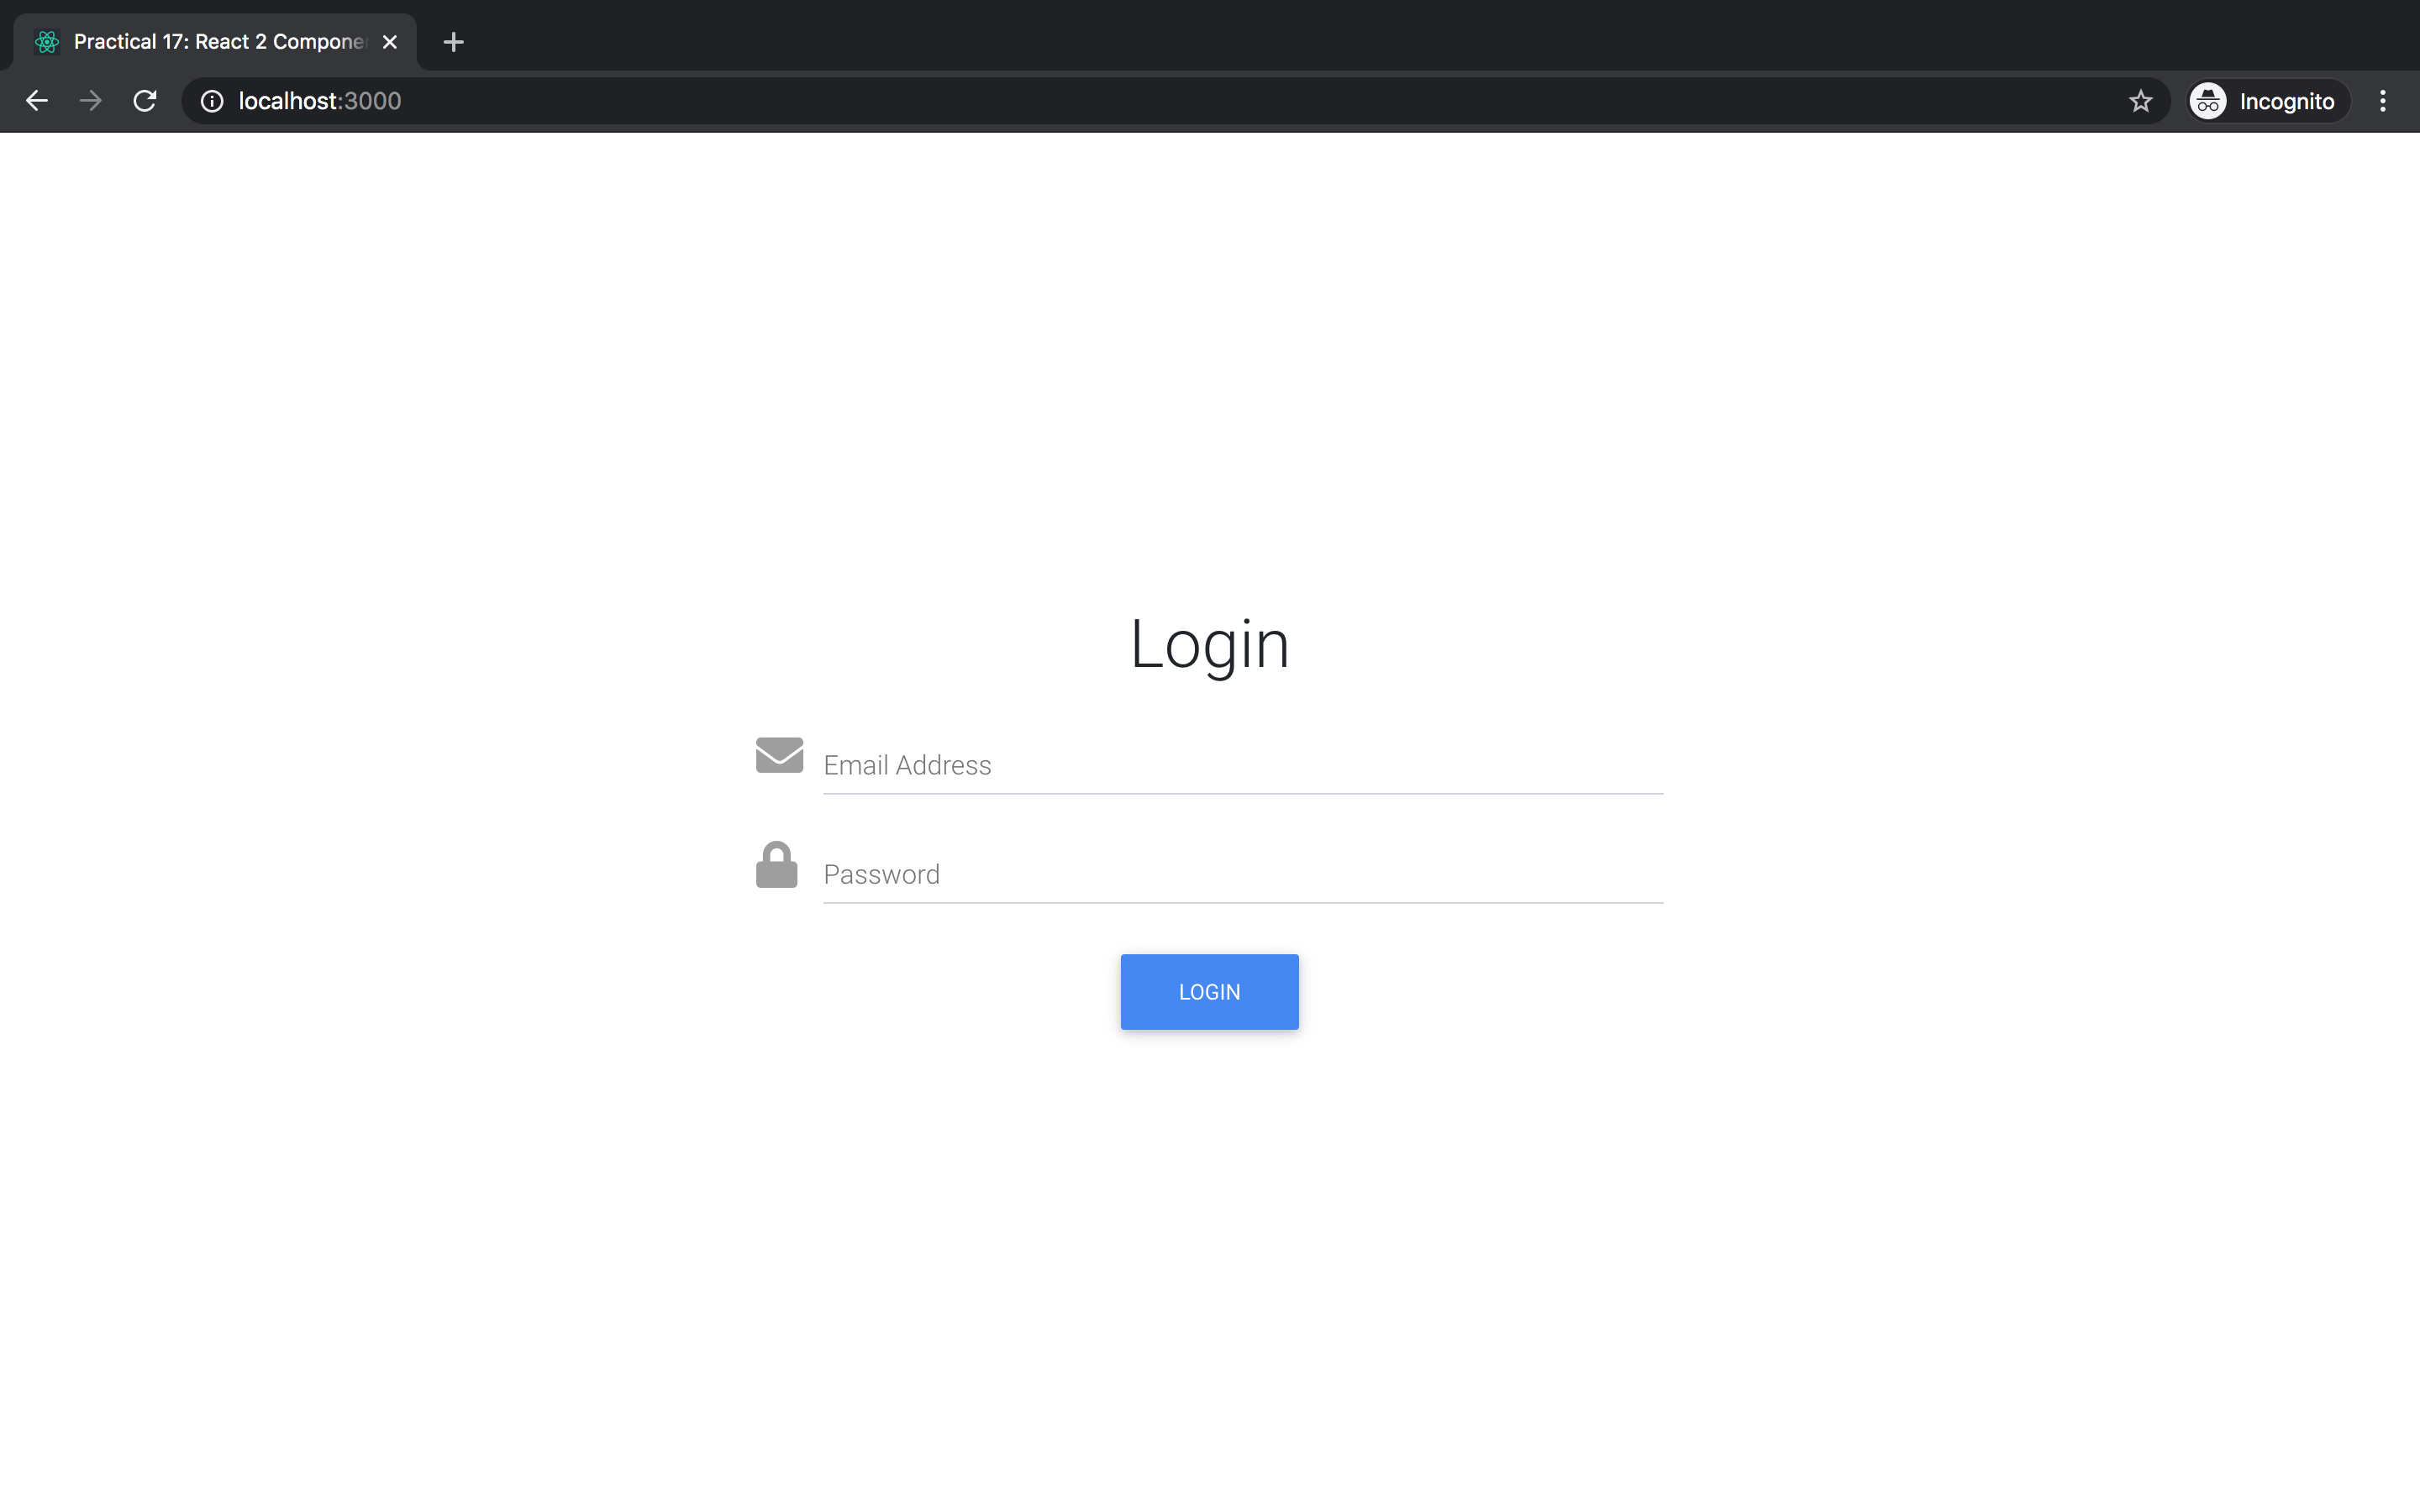
\includegraphics[width=175mm, height=105mm]{./img/17-expected-form-1.png}
  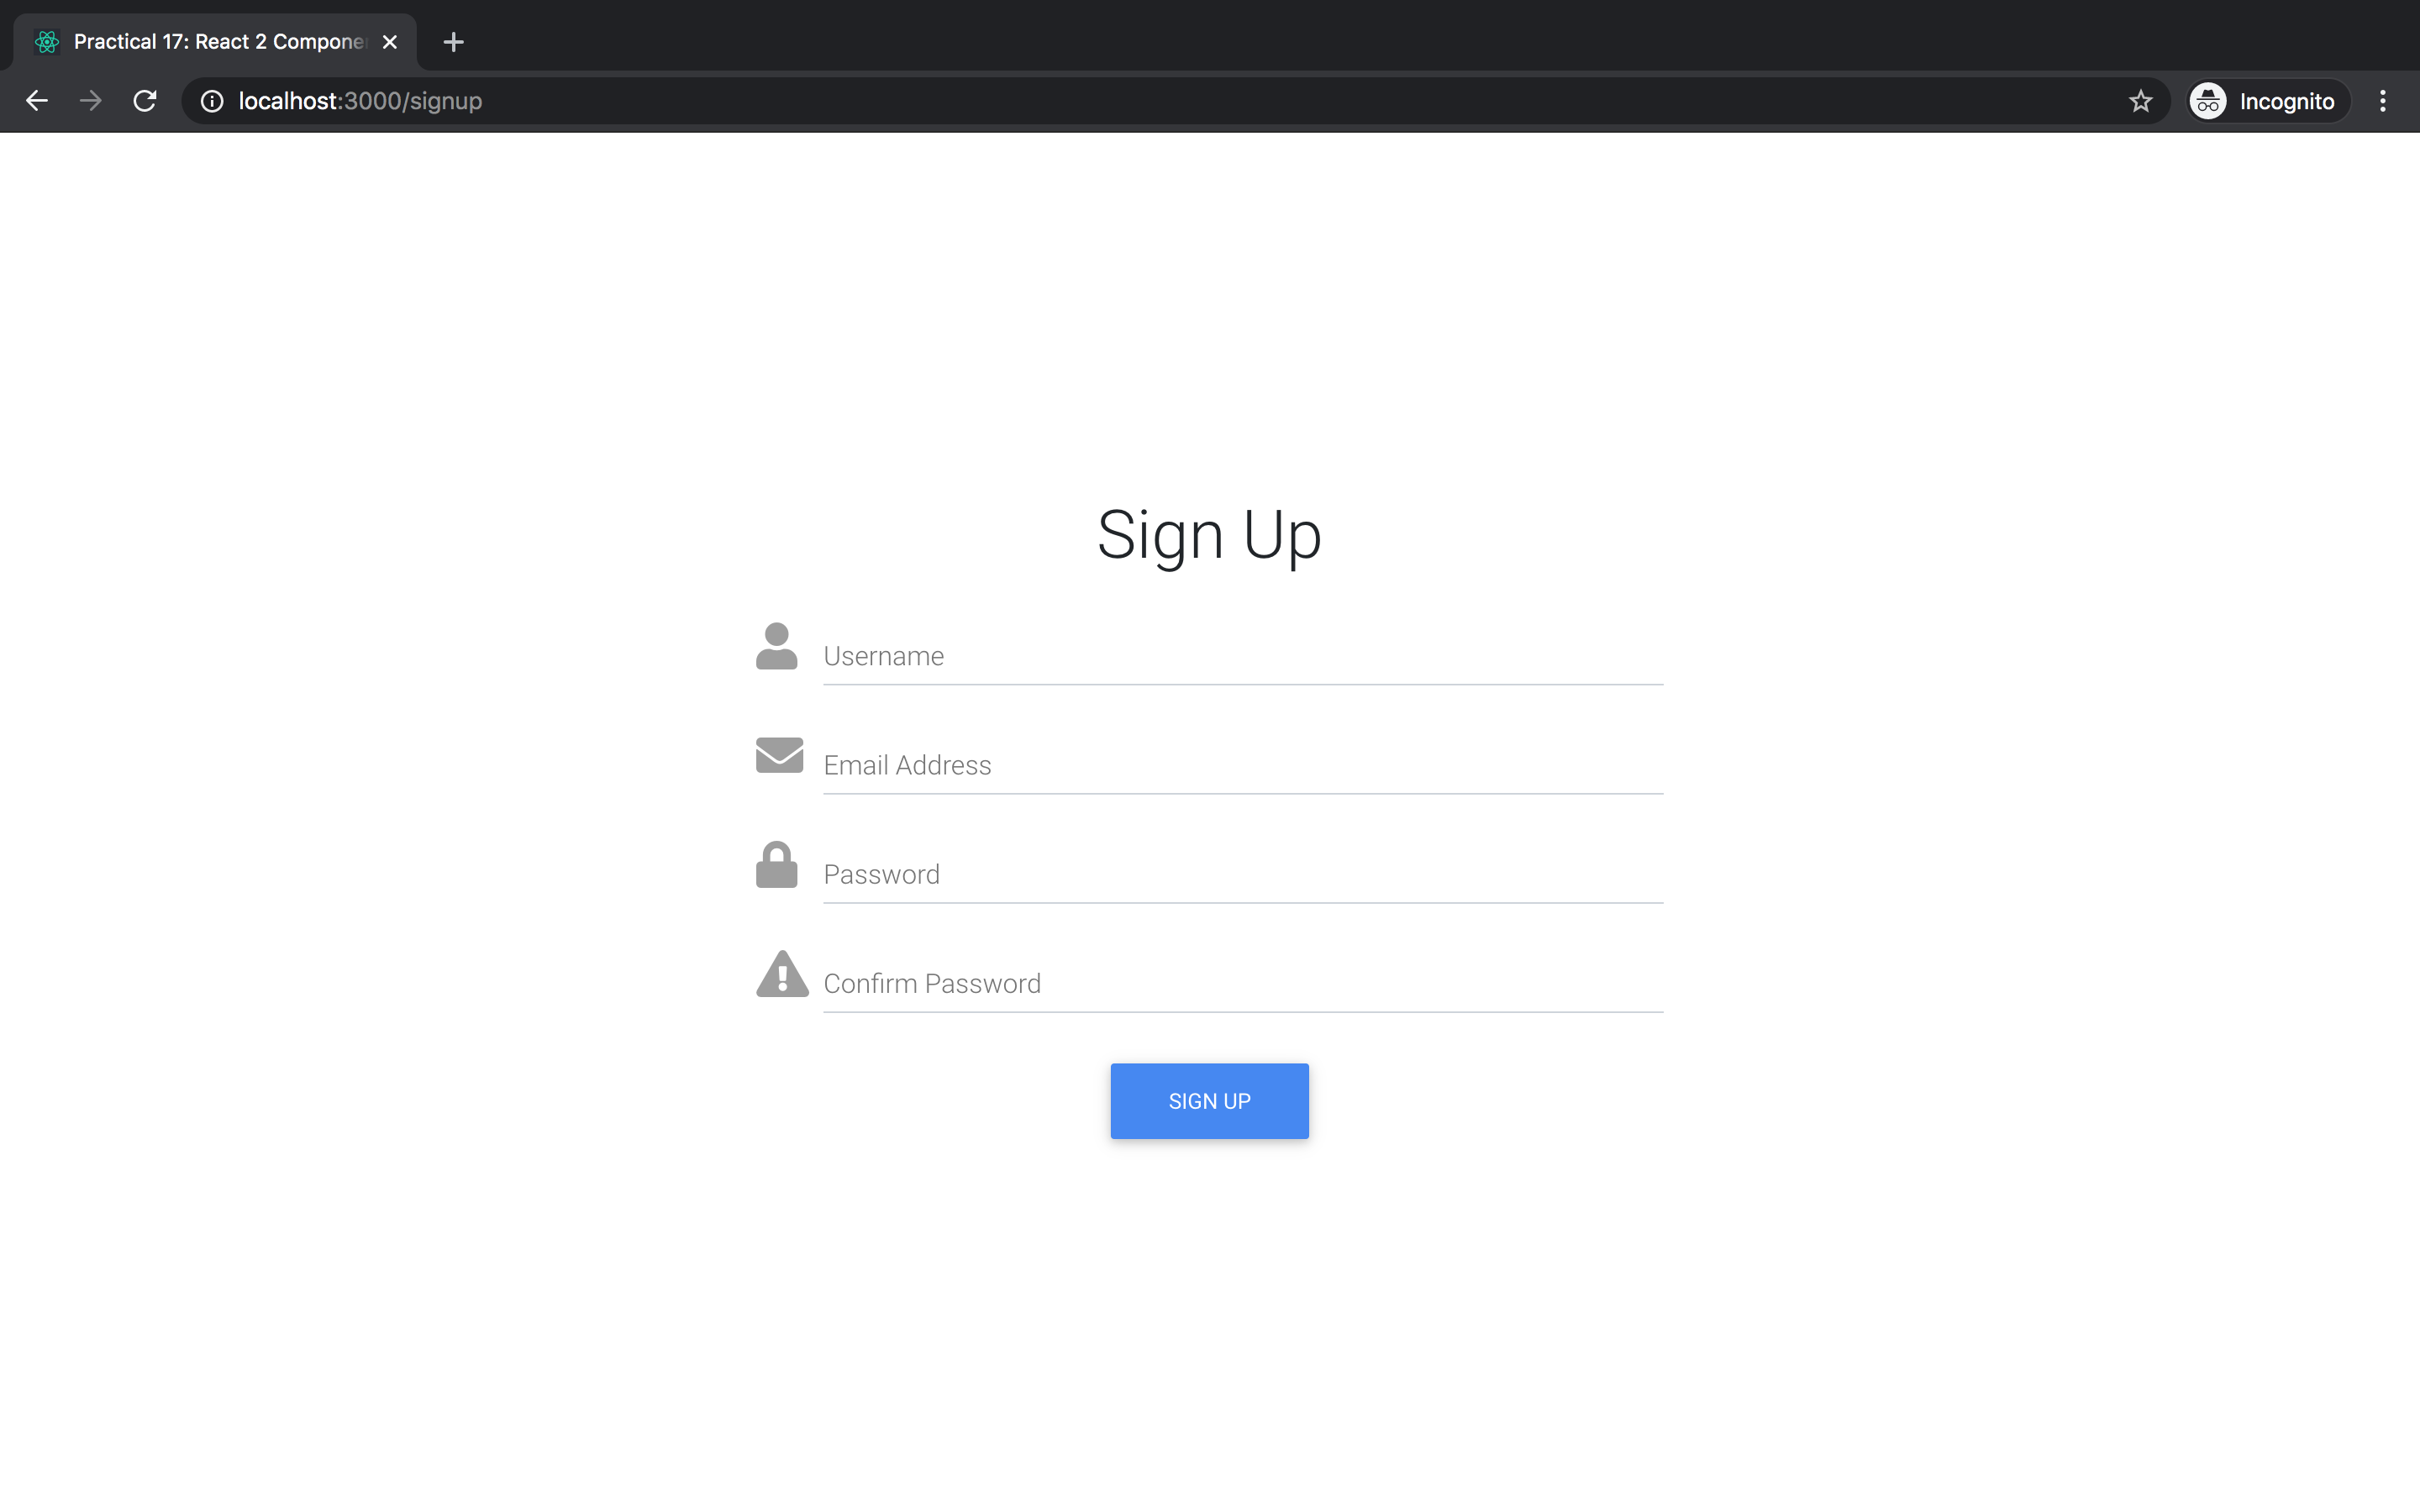
\includegraphics[width=175mm, height=105mm]{./img/17-expected-form-2.png}
\end{figure}

\begin{figure}[H]
  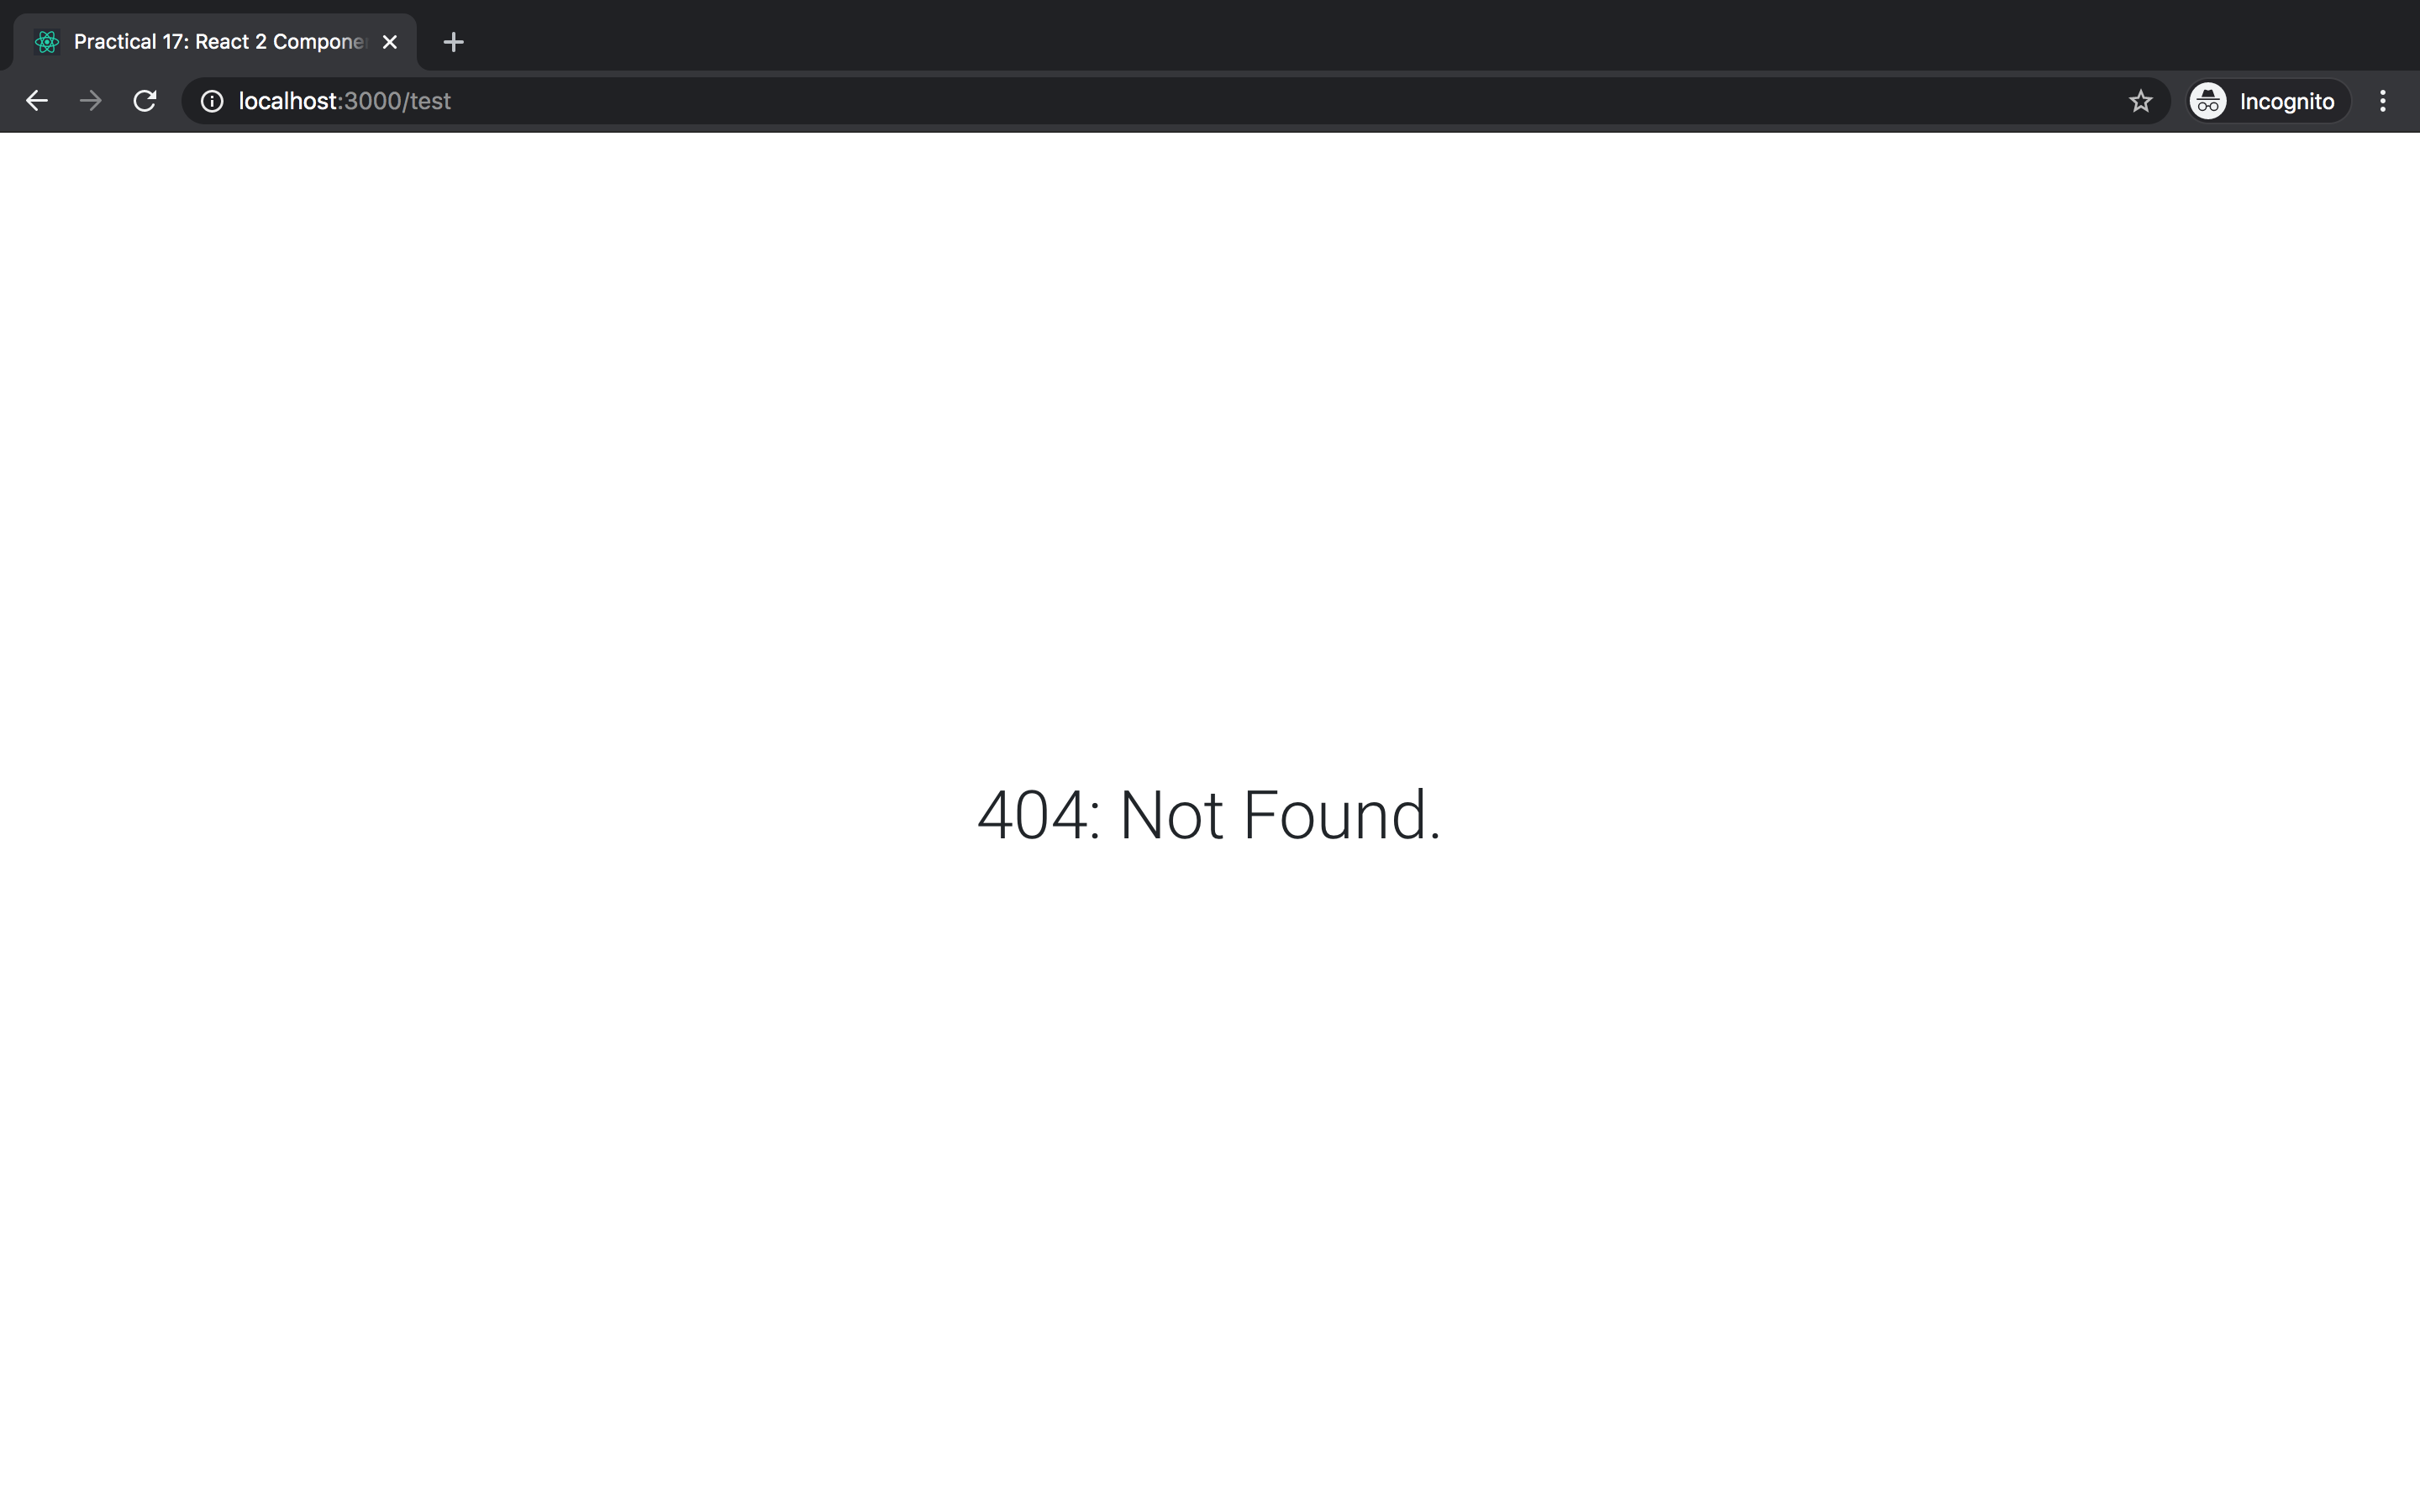
\includegraphics[width=175mm, height=105mm]{./img/17-expected-form-3.png}
\end{figure}

\textbf{Deployment link:} \href{https://int-app-dev-practical-17.herokuapp.com/}{https://int-app-dev-practical-17.herokuapp.com/} 

\subsection*{Resources} 
\begin{itemize}
  \item \href{https://mdbootstrap.com/}{Material Design for Bootstrap}
  \item \href{https://www.npmjs.com/package/mdbreact/}{Material Design for Bootstrap - npm}
  \item \href{https://reactrouter.com/web/guides/quick-start/}{React router DOM}
  \item \href{https://www.npmjs.com/package/react-router-dom/}{React router DOM - npm}
\end{itemize}
 
\end{document}